% =============================================
% 导言区
% =============================================
\documentclass{xjtureport}








% =============================================
% 正文区
% =============================================


\begin{document}

% ===导入实验报告封面==============================
\begin{titlepage}
	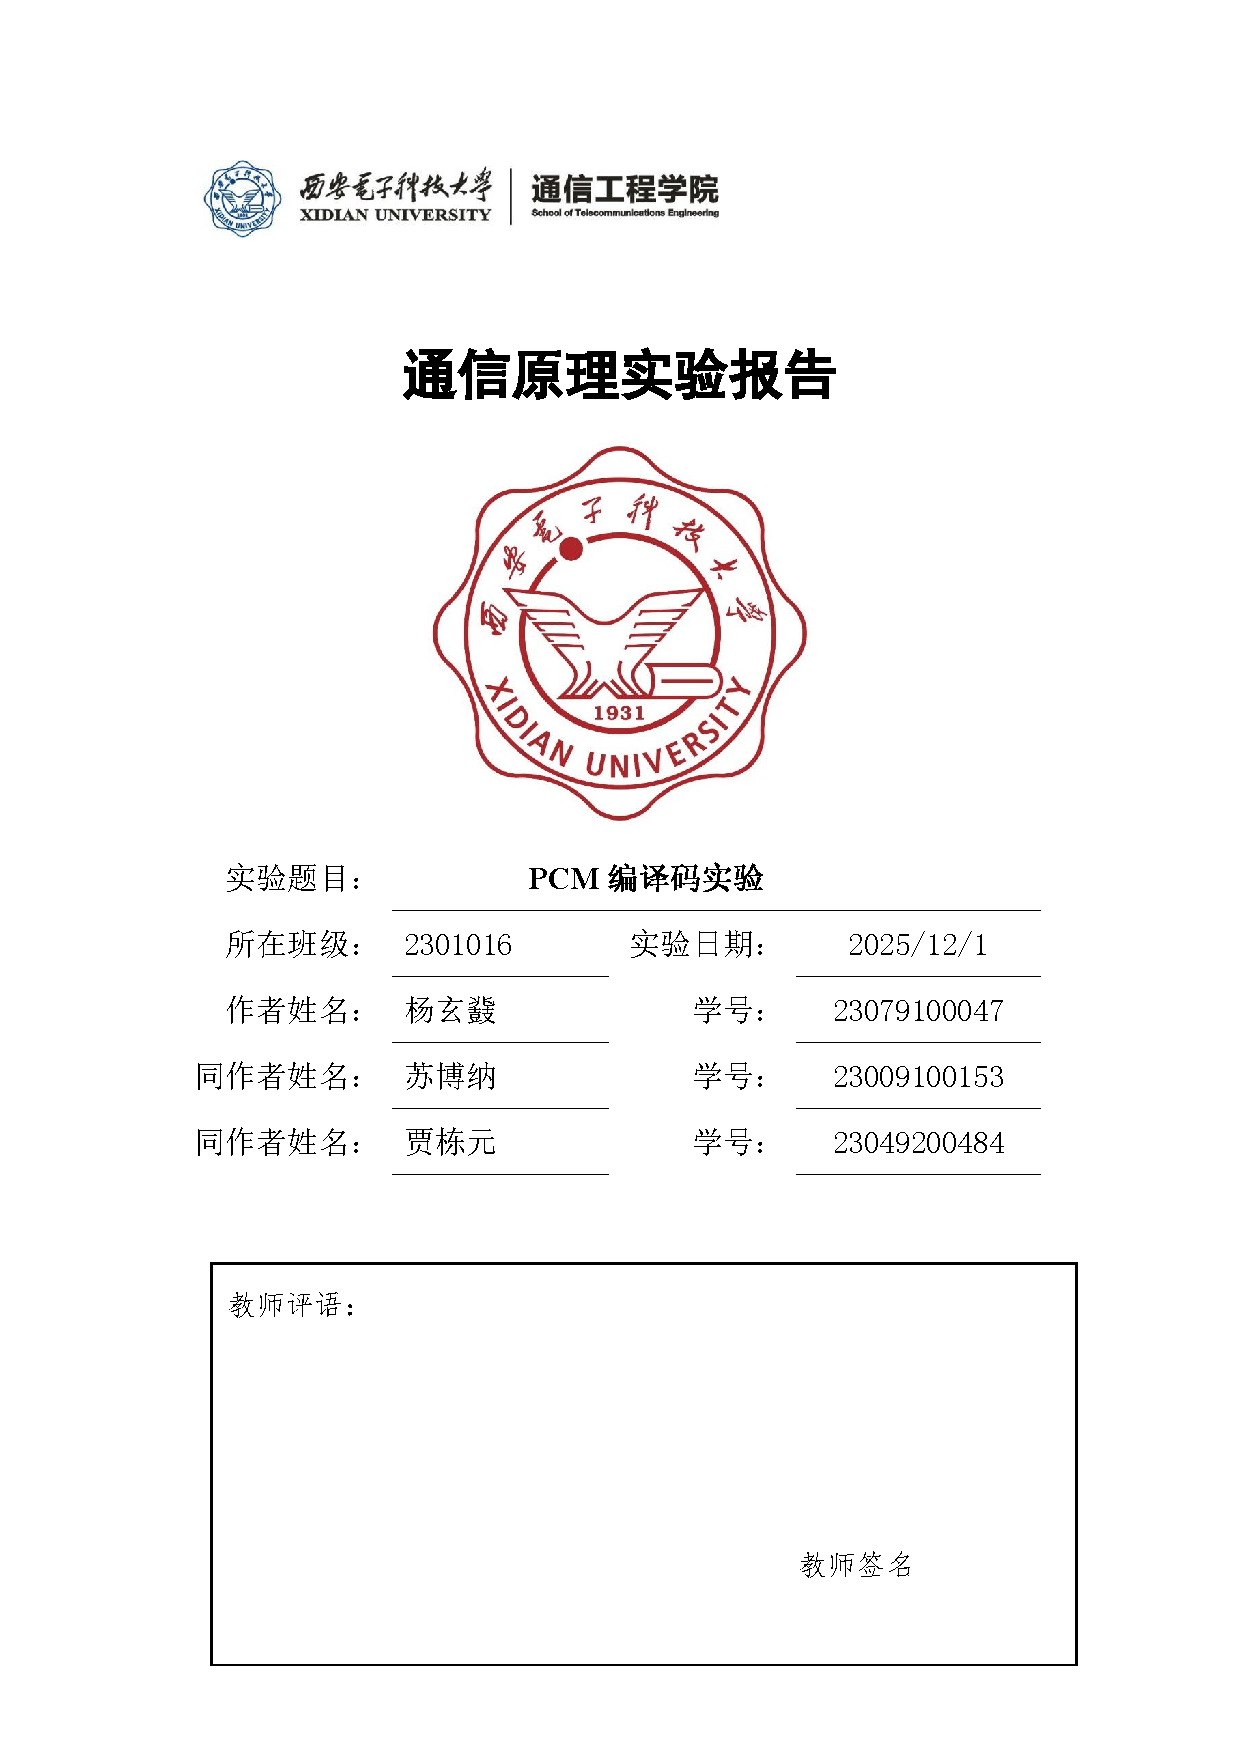
\includepdf[pages=-]{figures/实验4封面.pdf}
\end{titlepage}



% ===正文==============================


% 标题（一级居中）

\chapterinline{实验四： PCM编译码实验}

\section{实验目的}
（1）理解PCM编译码原理及PCM编译码性能；

（2）熟悉PCM编译码专用集成芯片的功能和使用方法及各种时钟间的关系；

（3）熟悉语音数字化技术的主要指标及测量方法。

\section{实验器材}

西电通信与实验专业平台（半实物仿真）。

\section{实验内容}

\subsection*{(1)原理验证}

	设置原始信号为：“正弦”，频率：1KHz，幅度设置指示为45

	  \begin{enumerate}[label=\roman*.]  % 二级编号：i., ii., iii., ...
		
		\item PCM串行接口时序观察
			
			输出时钟和帧同步时隙信号观测：用示波器同时观测并记录抽样脉冲信号2TP9和输出时钟信号2TP8，观测时以2TP9做同步
		
			\textbf{实验结果：}
			
			波形如图所示。CH1（黄色）为抽样脉冲 2TP9，呈低占空比脉冲序列；CH2（青色）为输出时钟 2TP8，在每个抽样脉冲周期内连续输出多个时钟脉冲。
			
			\begin{figure}[H]
				\centering
				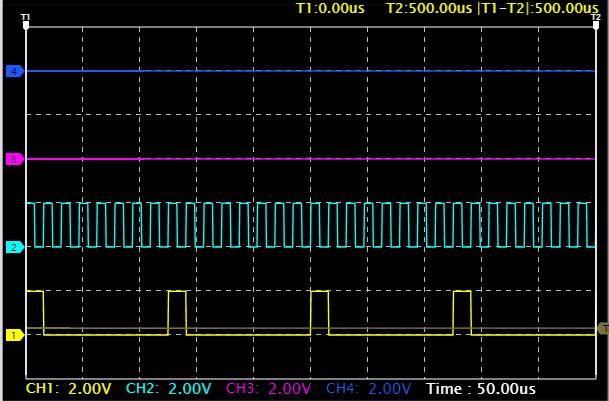
\includegraphics[width=0.5\linewidth]{figures/串行接口时序观察.png}
				\caption{抽样脉冲 2TP9 与输出时钟 2TP8 的时序波形}
			\end{figure}
			
			\vspace{3em}
		
		\item PCM串行接口时序观察
			
			抽样时钟信号与PCM编码数据测量：用示波器同时观测并记录抽样脉冲信号2TP9和编码输出信号2P6，观测时以2TP9做同步。
		
			\textbf{实验结果：}
			
			示波形如图所示。CH1（黄色）为抽样脉冲 2TP9，CH2（青色）为编码输出数据 2P6。可以看到编码数据在每个抽样脉冲之后开始输出，与抽样脉冲保持严格的时隙对应关系。
			
			\begin{figure}[H]
				\centering
				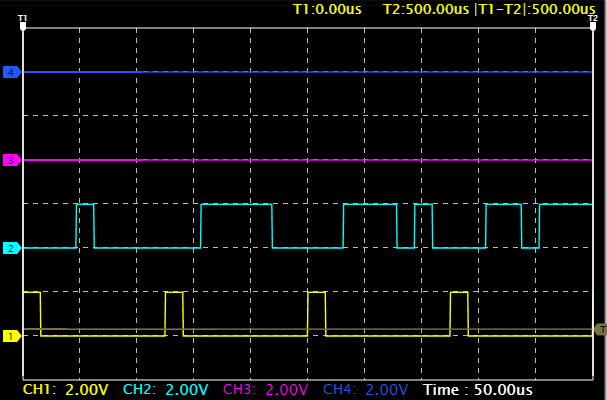
\includegraphics[width=0.5\linewidth]{figures/串行接口时序观察（抽样脉冲与编码输出信号）.png}
				\caption{抽样脉冲 2TP9 与编码输出数据 2P6 的时序关系}
			\end{figure}
			
			\textbf{分析：}
			
			编码输出信号 2P6 在抽样脉冲 2TP9 的下降沿之后稳定输出本次样值的 8 bit PCM数据，高位在前依次移出。数据电平变化与时钟、抽样脉冲严格对齐，说明编码器按帧同步节拍依次发送每个量化样点的编码结果，满足典型 PCM 串行输出时序特性。
			
			\vspace{3em}
			
		\item 在液晶观测 PCM 编码
		
		用鼠标点击 PCM 编译码框图右上角 “！” 号，液晶屏上会出现 PCM 编码解析图，我们可以观察模拟信号、抽样脉冲、量化值、编码值等相关波形和参数，根据实验原理研究量化值和编码值之间的对应关系。
		
			\textbf{实验结果：}
			
			实验中液晶显示界面如图所示。黄色曲线为输入的模拟正弦信号，绿色竖线为抽样瞬时刻度，蓝色数字为该抽样点对应的量化值（范围约为 $-960$ 至 $960$）。下方红色波形为相应的 8 bit PCM 编码序列，每个抽样点下方同时给出了相应的二进制编码，如 \texttt{00111110}、\texttt{10111011} 等，编码比特数固定为 8 位。。
			
			\begin{figure}[H]
				\centering
				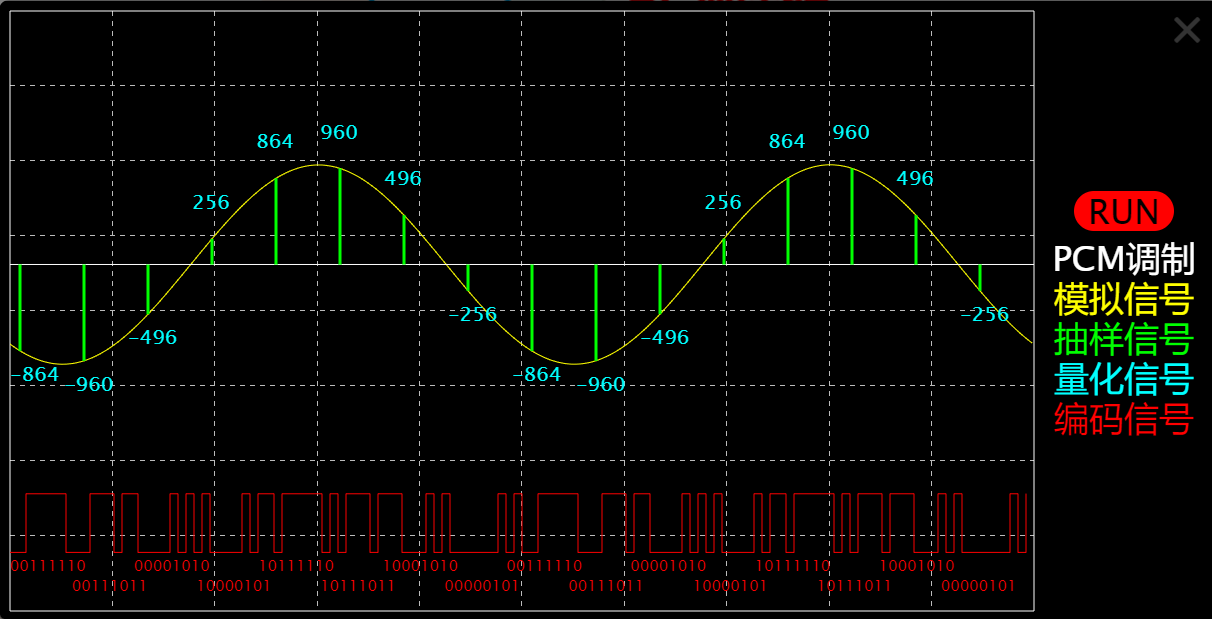
\includegraphics[width=0.6\linewidth]{figures/PCM编码解析图.png}
				\caption{液晶界面显示的模拟信号、量化值及 PCM 编码值}
			\end{figure}
			
			\textbf{分析：}
			
			液晶界面清晰展示了 A 律 13 折线的量化与编码流程：首先依据量化值符号确定极性码，其后根据量化值所在区间生成段落码，最后依量化值与段起始电平之差生成段内码。界面中各抽样点的量化值与其对应的 PCM 编码一一对应，验证了软件编码模块对 A 律压缩、分段量化与编码规则的正确实现。
		
			
			\vspace{3em}
		
		\item PCM编码输出数据观测
		
			\textbf{实验结果：}
			
			波形如图所示。可以观察到编码数据在每次抽样脉冲之后按照 8 bit PCM 格式依次输出，数据电平在时钟周期内保持稳定，形成典型的串行编码波形。
			
			\begin{figure}[H]
				\centering
				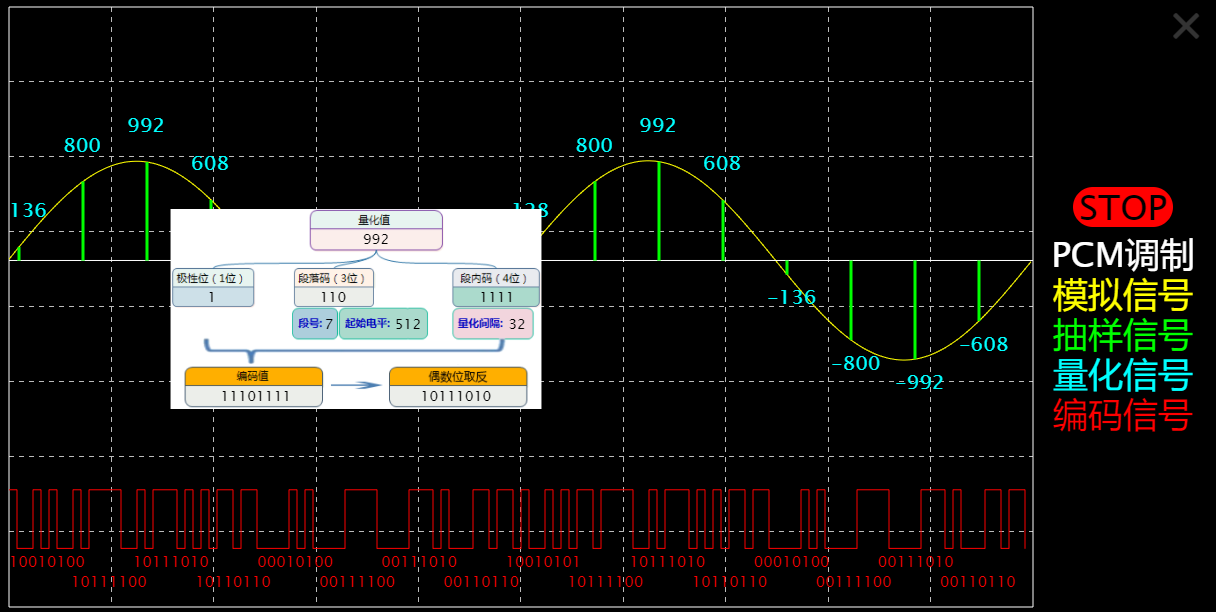
\includegraphics[width=0.6\linewidth]{figures/编码输出数据观测（液晶图）.png}
				\caption{2TP9 抽样脉冲与 2P6 编码输出数据的液晶屏观测波形}
			\end{figure}
			
			\vspace{3em}
		
		\item 用示波器同时观测抽样脉冲信号（2TP9）和编码输出数据端口（2P6），观测时以2TP9做同步。在示波器上读出一个编码样点值并记录波形，并和液晶上的相应编码数据进行比较。
			
			\textbf{实验结果：}
			
			\begin{figure}[H]
				\centering
				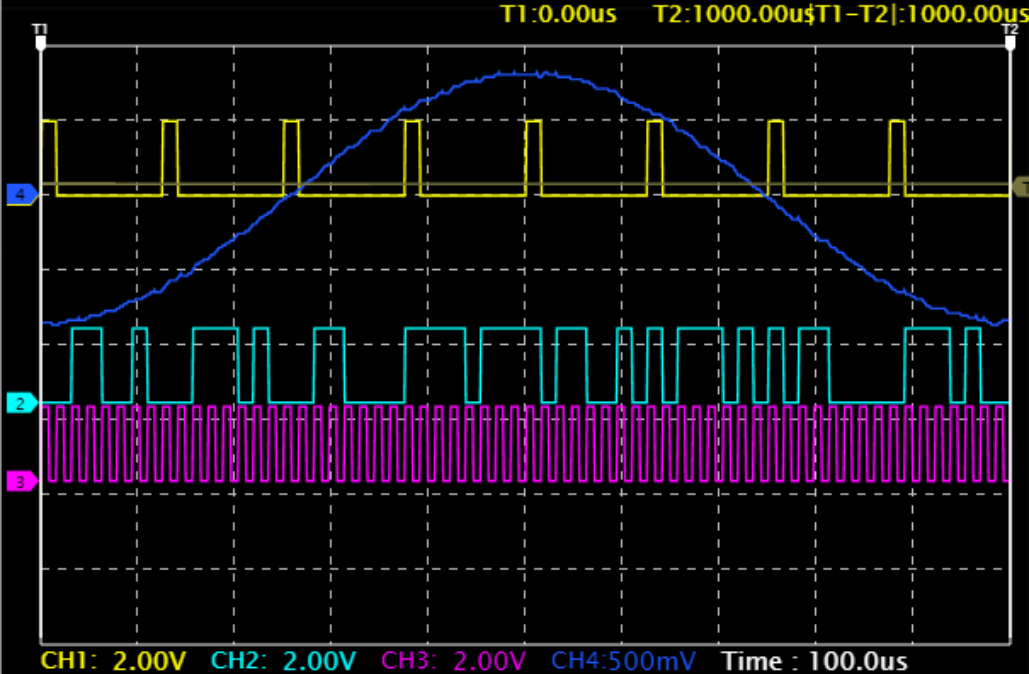
\includegraphics[width=0.6\linewidth]{figures/编码输出数据观测.png}
				\caption{2TP9 抽样脉冲与 2P6 编码输出数据的示波器观测波形}
			\end{figure}
			
			\textbf{分析：}
			
			在示波器上选取某一抽样点，可以读出编码输出 2P6 的 8 bit 串行比特序列。例如，对应液晶界面量化值为 960 的样点，其液晶显示的 PCM 原始编码为 \texttt{11101110}。根据 TP3057 的输出特性，实际串行输出的数据其偶数位会自动取反，因此示波器上观测到的编码比特序列为 \texttt{10111011}。两者之间满足“偶数位取反”的关系，说明软件编码与硬件串行接口输出保持一致，编码器工作正常。
			
			\vspace{3em}
			
		\item 数据分析：
		
			\begin{enumerate}[label=\alph*)]
				
				\item PCM 编码抽样脉冲信号与输出时钟的对应关系
				
				\textbf{答：}
				抽样脉冲 2TP9 的下降沿用于指示新一帧 PCM 数据的开始，其周期为 8\,kHz。输出时钟 2TP8 为连续的线路时钟，在每个抽样脉冲周期内提供 8 个比特位置的时隙。两者之间保持严格同步，抽样脉冲的下降沿作为帧同步基准，而输出时钟用于比特级串行移位输出。
				
				\vspace{3em}
				
				\item PCM 编码输出数据与抽样脉冲信号（数据输出与抽样脉冲沿）及输出时钟的对应关系
				
				\textbf{答：}
				PCM 编码数据 2P6 的输出总是在抽样脉冲 2TP9 的下降沿之后开始，按照输出时钟 2TP8 的节拍依次发送 8 位编码数据（高位在前）。每一个时钟周期对应一位编码值。需要注意的是，商用 PCM 编译码芯片在串行输出时会对偶数位自动取反，因此示波器上看到的比特序列与液晶显示的原始编码值之间存在“偶数位反转”的对应关系。
				
				\vspace{3em}
				
				\item PCM 编码规则是什么？
				
				\textbf{答：}
				本实验采用 A 律 13 折线 PCM 编码规则。每个抽样量化值首先根据正负确定极性码 C1；随后根据量化值所在段落确定三位段落码 C2C3C4；最后根据量化值与段起始电平之间的差值确定四位段内码 C5C6C7C8。最终形成 8 位 A 律 PCM 码字。液晶中可以看到未反相的原始编码和偶数取反后的编码，而串行输出端则对偶数位执行反相处理。
				
				\vspace{3em}
			\end{enumerate}
			
		\end{enumerate}
		
\subsection*{(2) PCM译码观测}

用示波器同时观测输入模拟信号 2P7 和译码器输出信号 7P8，定性观测编译码前后波形（1\,kHz、2\,Vpp）的关系：质量、电平。

\textbf{实验结果：}

实验波形如图所示。CH1（黄色）为输入模拟信号 2P7，CH2（青色）为译码后输出信号 7P8。可以看出，两者均为近似相同频率的正弦波，译码后的波形整体保持输入信号的幅度与形状，只在细节上略显平滑。

\begin{figure}[H]
	\centering
	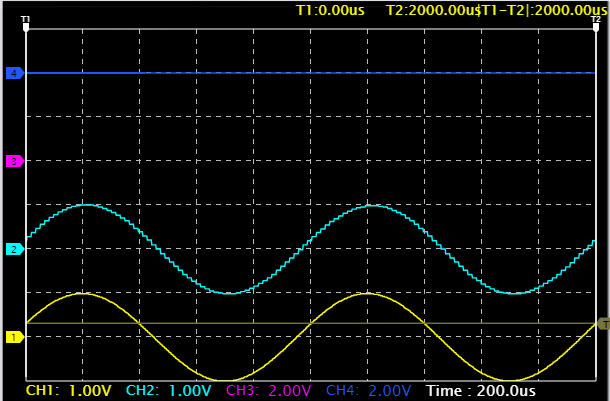
\includegraphics[width=0.6\linewidth]{figures/PCM译码观测.png}
	\caption{输入信号 2P7 与译码输出信号 7P8 的示波器观测波形}
\end{figure}

\textbf{分析：}

由示波器波形可以看出，译码输出 7P8 的频率与输入信号 2P7 一致，电平基本不变，且波形细节上呈现一定的“阶梯状/锯齿感”，不如输入正弦波那样平滑。这是由于 PCM 编译码过程中存在量化误差以及译码端采用保持电路加有限阶低通滤波器进行重构的结果：量化使信号幅度只能取有限个离散电平，译码后形成阶梯状波形，实际低通滤波器又无法完全消除这些高频成分，因此在输出波形上即可观察到轻微的锯齿失真。总体而言，信号的主频率和波形形状仍能较好保持，表明 PCM 编译码链路工作正常。

\subsection*{(3) 数据记录}

\subsubsection*{1.定性描述 PCM 编译码的特性、编码规则，并填下表}

\textbf{PCM 编译码的特性、编码规则：}

PCM 编译码的基本过程包括：对模拟信号进行抽样、量化并按照 A 律 13 折线规则进行压缩编码。
对于每个抽样样值，首先根据其符号确定 1 位极性码，随后根据量化值所在区段确定 3 位段落码，
最后根据该段内的相对电平确定 4 位段内码，从而构成 8 位 A 律 PCM 编码。
编码输出采用串行方式发送，在每个抽样脉冲下降沿之后依次输出 8 bit（高位在前），
且实际串行输出端会对偶数位进行反相处理。

\begin{table}[H]
	\centering
	\small
	\begin{tabular}{|c|cccccccc|}
		\hline
		频率：1kHz & 样点1 & 样点2 & 样点3 & 样点4 & 样点5 & 样点6 & 样点7 & 样点8 \\
		幅度：2Vpp &       &       &       &       &       &       &       &       \\
		\hline
		量化值     & 400 & 928 & 928 & 368 & -416 & -928 & -928 & -368 \\
		\hline
		编码值（原始PCM码） & 
		11011001 &
		11101101 &
		11101101 &
		11010111 &
		01011010 &
		01101101 &
		01101101 &
		01010111 \\
		\hline
	\end{tabular}
	\caption{PCM 编码样点的量化值与编码值记录（未反相原始编码）}
\end{table}

\subsubsection*{2.描述 PCM 编码串行同步接口的时序关系。}

PCM 编码的串行同步接口由帧同步脉冲 FS（2TP9）、线路时钟 BCLK（2TP8）以及串行编码数据 DOUT（2P6）三部分组成，其时序关系如下：

（1）帧同步脉冲 FS 的下降沿标志着一个新的采样周期开始，是 PCM 编码器输出 8 bit 码字的起始基准。

（2）在 FS 下降沿之后，编码数据 DOUT 在随后的 8 个 BCLK 时钟周期内依次移出，每个时钟周期传输 1 bit，且高位在前（MSB first）。

（3）BCLK 为连续时钟，用于对串行数据进行比特级同步；FS 脉冲仅用于帧同步，不作为比特时钟使用。

（4）实验所用编码芯片在线路输出端对偶数位进行反相处理，因此示波器上观测到的比特流与原始 PCM 编码之间存在“偶数位取反”的对应关系。

综上，PCM 串行同步接口的时序结构清晰：FS 指示帧边界，BCLK 决定比特节拍，8 位 PCM 码字在一个 FS 周期内按照 BCLK 时钟顺序传输完成。

\subsubsection*{3.填下下表，并画出 PCM 的频响特性。}

\begin{table}[H]
	\centering
	\begin{tabular}{|c|cccccccc|}
		\hline
		输入频率（Hz） & 200 & 500 & 800 & 1000 & 2000 & 3000 & 3400 & 3600 \\
		\hline
		输出幅度（V） & 0.20 & 0.80 & 1.10 & 1.00 & 1.00 & 1.00 & 0.44 & 0.04 \\
		\hline
	\end{tabular}
	\caption{PCM 编码系统的频响测量结果}
\end{table}

为了便于观察频率响应的变化趋势，基于上述实验数据绘制 PCM 系统的幅频特性曲线，
结果如图所示。

\begin{figure}[H]
	\centering
	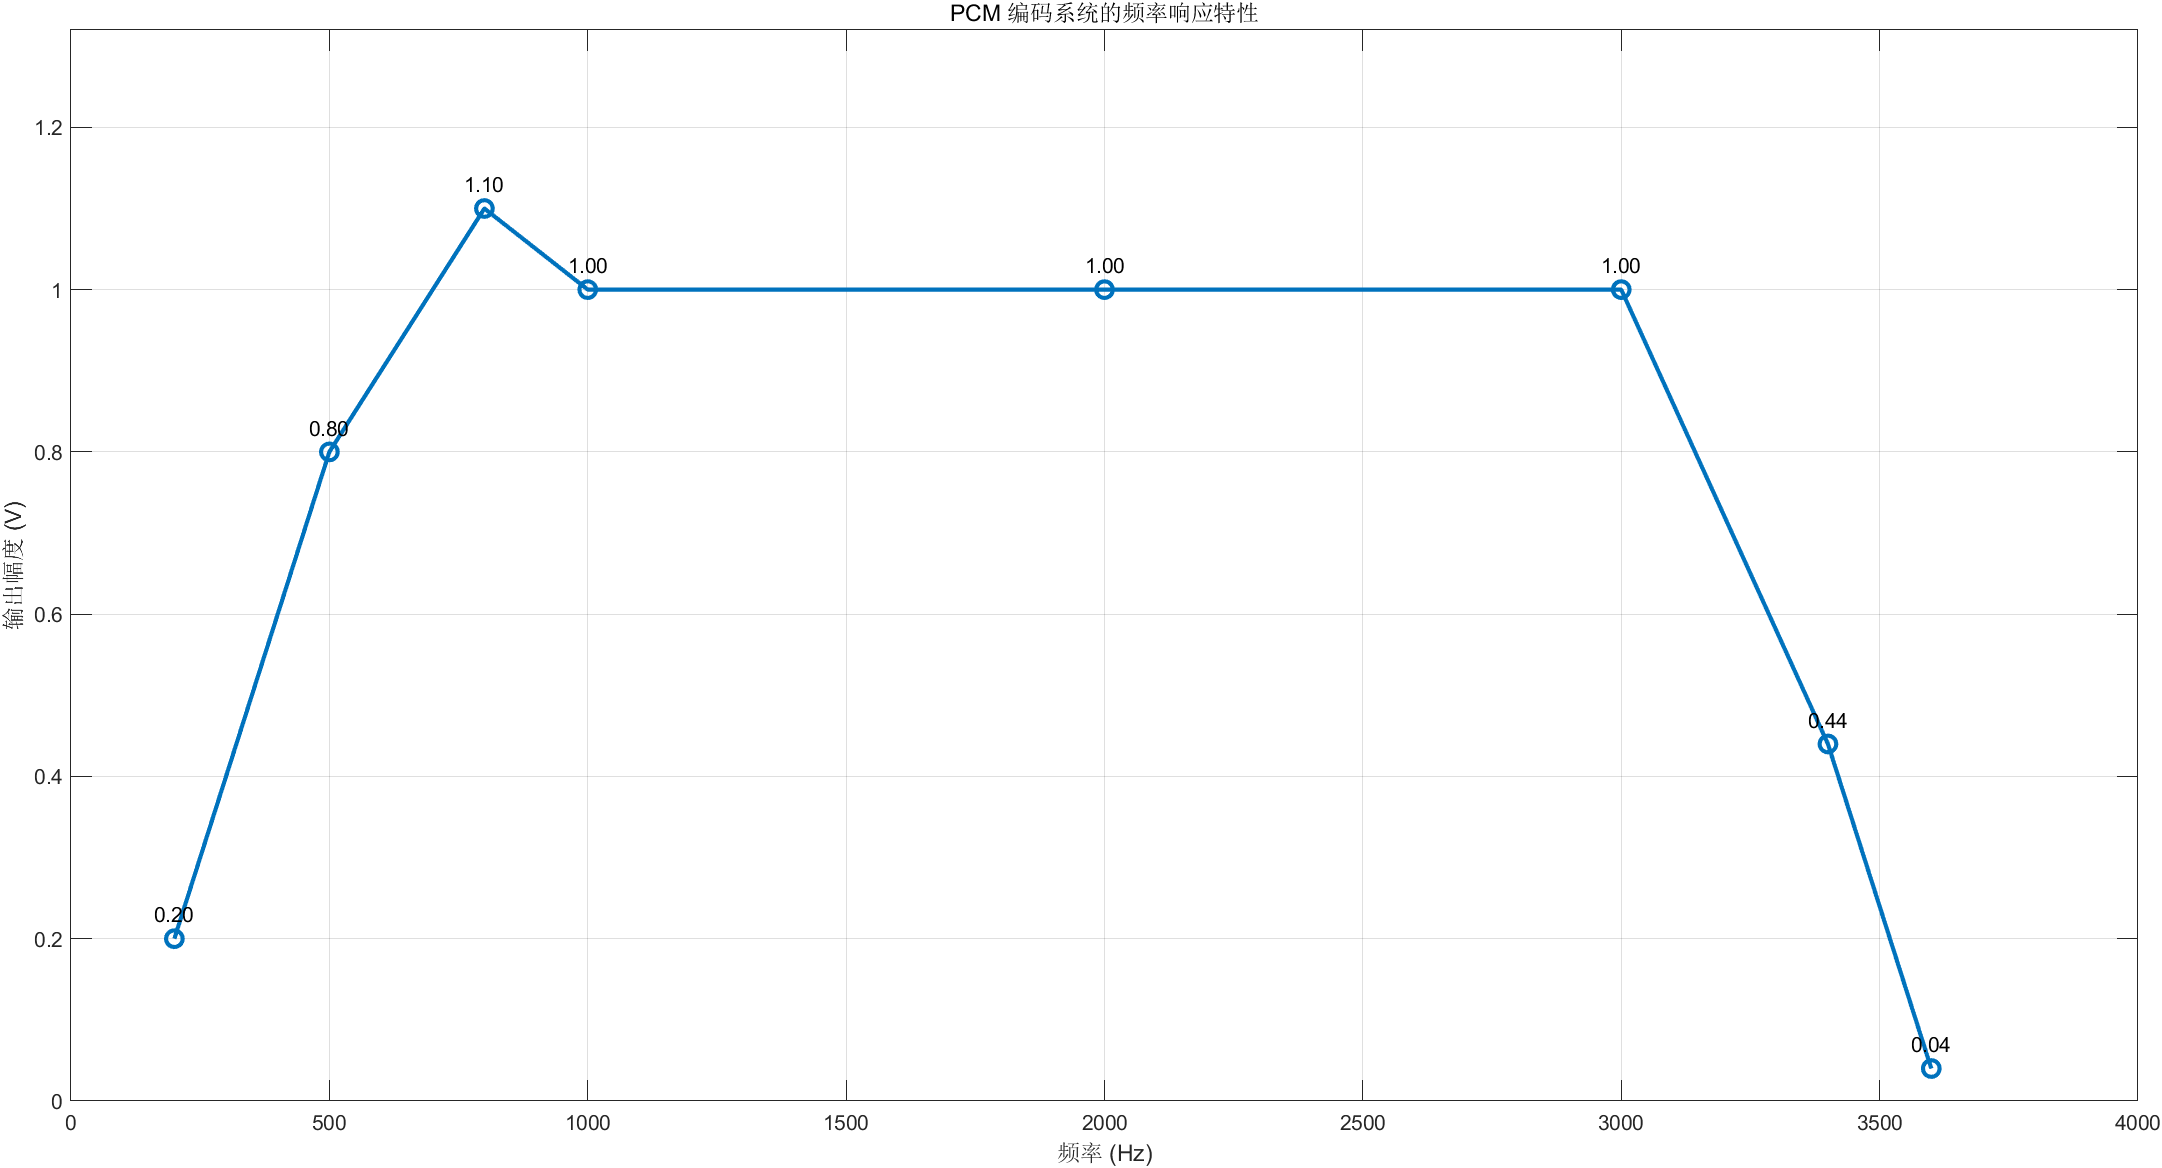
\includegraphics[width=0.6\linewidth]{figures/频率响应.png}
	\caption{PCM 系统的幅频响应曲线}
\end{figure}


\subsubsection*{4.填下下表，并画出 PCM 的动态范围：}

\begin{table}[H]
	\centering
	\begin{tabular}{|c|ccccccc|}
		\hline
		输入幅度（V） & 0.1 & 0.2 & 0.5 & 1 & 2 & 3 & 4 \\
		\hline
		输出幅度（V） & 0.08 & 0.20 & 0.50 & 1.00 & 2.00 & -- & -- \\
		\hline
	\end{tabular}
	\caption{PCM 系统的动态范围测量结果}
\end{table}


\textbf{分析：}

从表中可以看出，当输入幅度在 $0.1\sim2\,\mathrm{V}$ 范围内时，输出幅度基本与输入幅度成线性对应关系，
说明 PCM 编译码链路在该范围内能够较好保持幅度特性。

当输入电平继续增大（超过 $2\,\mathrm{V}$）时，系统进入饱和区，
由于采样前模拟前端以及 ADC 输入范围的限制，输入信号已无法被完整采样，
因此在 $3\,\mathrm{V}$ 和 $4\,\mathrm{V}$ 时无法获得有效输出。

整体来看，PCM 编码系统的可用动态范围约为 $0.1\sim2\,\mathrm{V}$。

PCM 的动态范围曲线如图所示：

\begin{figure}[H]
	\centering
	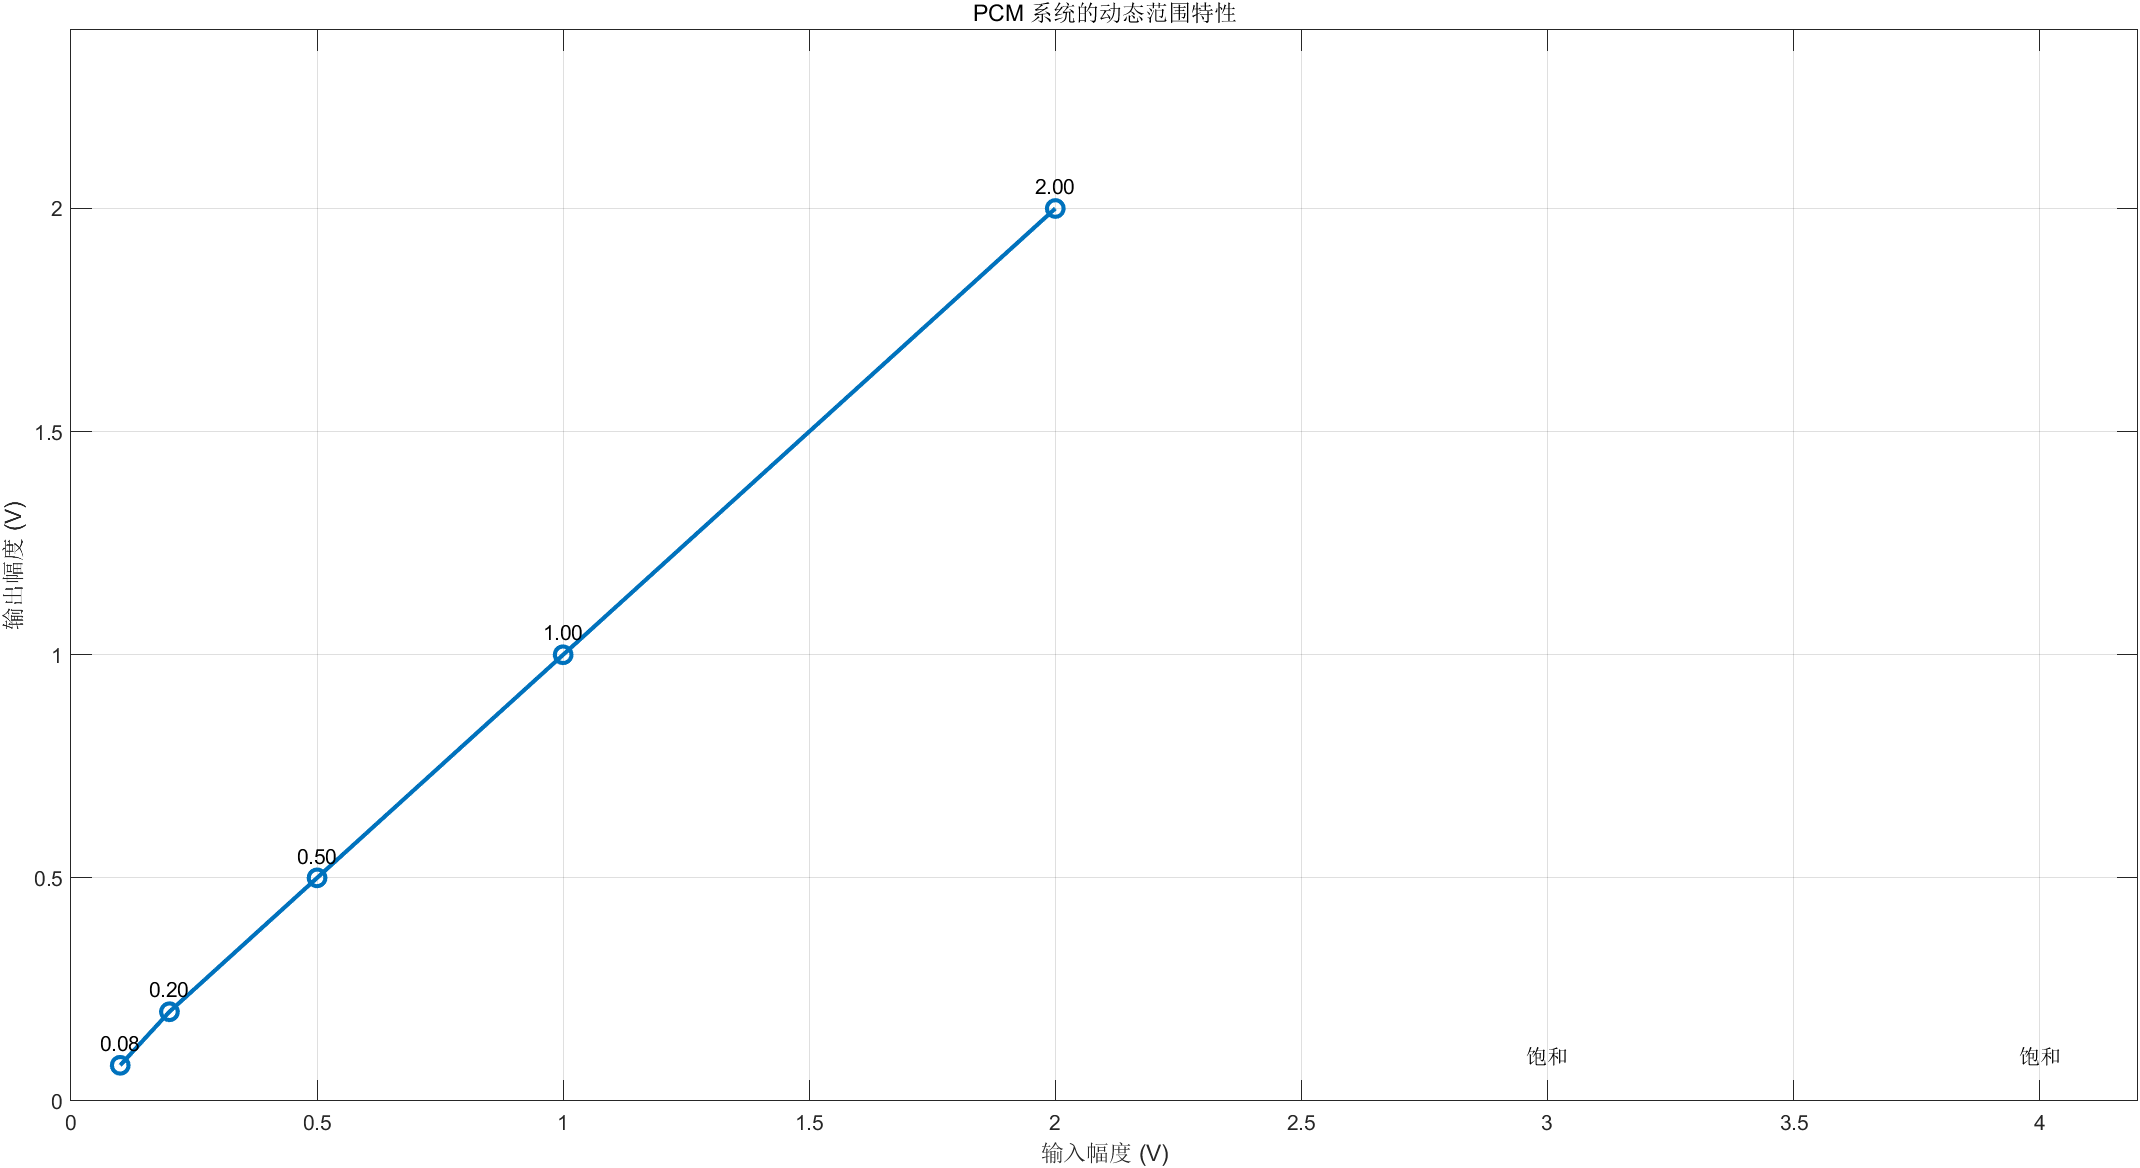
\includegraphics[width=0.5\linewidth]{figures/PCM动态范围.png}
	\caption{PCM 编码系统的动态范围曲线}
\end{figure}


\section{问题回答}

\subsection*{1. 输入信号为0Vpp时，PCM编码数据是多少？为什么？}

\textbf{答：}
当输入信号为 0Vpp 时，所有采样点的瞬时幅度均为零，对应的量化值为 0。
根据 A 律 13 折线 PCM 编码规则，量化值为 0 属于极性为负（C1=0）、段落码为 000、段内码为 0000，
因此其 PCM 原始编码为 \texttt{00000000}。
在实际串行输出端，由于 TP3057 对偶数位进行反相处理，
示波器上观察到的比特序列仍为全零，因此最终输出也表现为 \texttt{00000000}。


\subsection*{2. 简述PCM编码流程}

\textbf{答：}
PCM 编码流程包括以下步骤：

(1) 对模拟信号进行带限处理，使其限定在语音带宽内（300--3400Hz）。

(2) 以固定采样频率（本实验为 8kHz）对模拟信号抽样，得到离散的采样幅度。

(3) 将采样幅度进行量化，本实验采用 A 律 13 折线压扩量化，将连续幅值映射到 256 个量化级。

(4) 根据量化值的极性、所属段落以及段内位置生成 8 bit PCM 编码（1 位极性码、3 位段落码、4 位段内码）。

(5) 编码数据按 MSB→LSB 顺序在一个帧同步脉冲周期内串行输出，并由线路时钟提供位同步。
实际硬件输出端会对偶数位自动反相以满足标准 PCM 接口格式。

以上完成了模拟信号向数字 PCM 符号序列的编码过程。


\section{心得体会}

通过本次实验，我对 PCM 编译码的全过程有了更加直观而深入的理解。通过实验平台的波形观测，
我第一次清晰地看到模拟信号的抽样脉冲、量化值以及对应的 PCM 八位编码之间的关系，
也体会到 A 律压缩在语音信号中的实际应用。

在编码端，通过观察抽样脉冲与输出时钟的时序，我理解了 PCM 串行同步接口的工作机制；
通过对比液晶显示的原始编码与示波器上串行输出的反相编码，
也进一步认识到商业 PCM 接口中偶数位反转的原因及作用。

在译码端，通过对输入与输出波形的对比，我看到了量化噪声和低通重构滤波器对信号形状的影响，
输出信号虽然整体保持了原始波形的特征，但在细节上存在轻微失真，
这与理论分析完全一致。此外，频响测量与动态范围实验也让我认识到 PCM 系统并非理想线性系统，
其有效工作带宽、动态范围会受到采样率、滤波器和量化器精度等多方面限制。

总体而言，本次实验不仅加深了我对 PCM 编译码原理的理解，
也提升了我对“理论—系统实现—实际观测”之间关系的认识。
通过操作仪器、分析波形和整理数据，我对通信系统中数字化处理的重要性和实际实现细节有了更全面的体会。


\end{document}